\subsection{Pulssensorer}
Kroppens puls kan detekteres på en række forskellige måder, heriblandt elektrisk, optisk, akustisk og mekanisk eller magnetisk.\cite{PhuaLissorguesMercier2009} 
\newline
Elektriske pulssensorer, måler pulsen ved elektrisk kontaktflade mellem sensor og person gennem elektroder. Pulsen detekteres ved de elektriske pulssensorer som forskellen i den elektriske ladning. Udfaldet af målingerne er subjektive, da de kan variere efter personens kropsvæsker såsom blod eller olier i huden.\cite{PhuaLissorguesMercier2009} 

Optiske pulssensorer registrere puls gennem lys. En rød LED sender lys, som passerer huden og blodåren. Noget af lyset absorberes af hæmoglobinen i blodet, hvorefter en fotodiode opfanger mængden af det resterende lys. Jo mere blod der er i åren, jo mindre lys bliver tranmitteret. Outputtet fra pulssensoren er spejlvendt af det lys der opfanges, så signalet giver udslag der stemmer overens med mængden af blod. Denne type sensor bruges ofte i fingerspidsen eller på tåen.\cite{PhuaLissorguesMercier2009,SrinivasReddySrinivas2006} 

Akustisk opfangelse af puls sker gennem et stetoskop. Dette er en enhed hvor lægen opfanger lyden fra hjertet gennem patientens bryst, og derudfra bestemmer pulsen.\cite{PhuaLissorguesMercier2009} 

Mekanisk kan pulsen opfanges ved brug af at piezo-elektrisk materiale, som presses mod huden, og opfanger presset fra hjerteslagene eller pulsen.\cite{PhuaLissorguesMercier2009} 

En anden metode er at placere magneter på kroppen, hvorved blodmolekylerne polariseres. Derefter kan potentialeforskellen registreres gennem elektroder tæt ved det pålagte magnetfelt.\cite{PhuaLissorguesMercier2009}

\subsubsection{Registrering af puls}
Pulsen er angivet som forskellen i det systoliske og diastoliske blodtryk som slag per minut. Pulsen kan måles menuelt ved at placere to fingre over en arterie, og derefter tælle hvor mange slag der er i minuttet. Hyppigst måles pulsen fra radial arterien på håndleddet eller på halsen, men enhver arterie der kan mærkes, kan bruges til at måle pulsen ved, se \figref{pulsmaaling}. 

\begin{figure}[H]
	\centering
	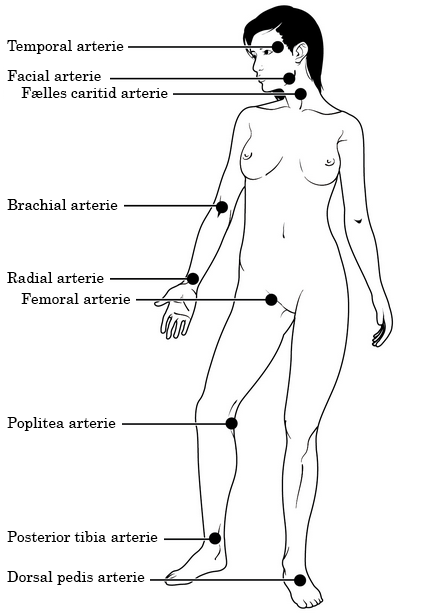
\includegraphics[scale=0.6]{figures/bProblemloesning/puls.png}
	\caption{På figuren ses steder det er muligt at måle puls.\citep{CNX2016}}
	\label{fig:sensor_placering}
	\end{figure}
	


